\newpage
\subsection{Partition::removeCard(Card) - The visual syntax}
\visHeader
\hypertarget{remCard vis}{}

\begin{itemize}

\item[$\blacktriangleright$] In Enterprise Architect (EA), open the main diagram (double-click in the project browser) and carefully do the following: (1) \emph{Click once} on
\texttt{Partition} to select it, then (2) \emph{click once} on the method \texttt{removeCard} to choose it (Fig.~\ref{fig:sdm_start}). (3) \emph{Double-click}
on the chosen method to indicate that you want to implement it.

\begin{figure}[htp]
\begin{center}
  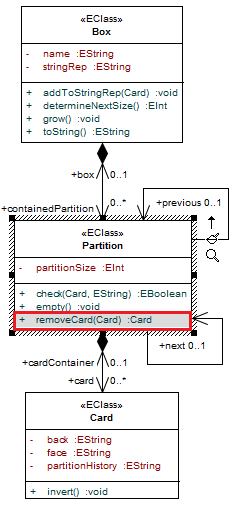
\includegraphics[width=0.4\textwidth]{ea_openMethodActivity}
  \caption{Double-click a method to implement it {\bf update image; missing card.method, partition.attrib} }  
  \label{fig:sdm_start}
\end{center}
\end{figure}
 
\item[$\blacktriangleright$] If you did everything right, a new \emph{activity diagram} should be created and open in a new tab with a cute little \emph{start node} 
labelled with the signature of the method (Fig.~\ref{fig:sdm_skeleton}).  

\item[$\blacktriangleright$] Inspect your project browser and note that an \texttt{<<SDM Activity>>} container has been created for the method
\texttt{removeCard} to contain the diagram. If you're at any time unhappy with an SDM\footnote{As you might have already noticed, we use ``SDM'' interchangeably
to mean our graph transformation language or a concrete transformation (a story model) used to implement a method and consisting of an activity diagram and a
pattern in each story node. This will all be explained in detail.}, you can always delete the appropriate container in the project browser and start from
scratch, following the steps described previously to create a skeleton for a new SDM. 

\item[$\blacktriangleright$] Also note the new toolbox \texttt{SDM} that has been automatically opened up for the diagram and placed to the left above the 
common toolbox.

\begin{figure}[htp]
\begin{center}
  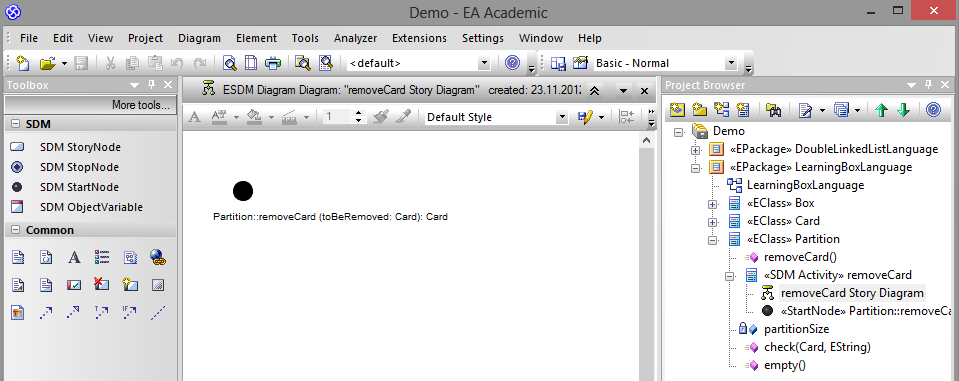
\includegraphics[width=0.9\textwidth]{ea_generatedSDMDiagram}
  \caption{Generated SDM diagram and start node {\bf update}}  
  \label{fig:sdm_skeleton}
\end{center}
\end{figure}

\item[$\blacktriangleright$] One of the first things you'll notice is a small anchor.. double click this to be taken back to the source diagram, the anchored
metamodel.

\item[$\blacktriangleright$] Choose the start node, and note the small black arrow that appears (Fig.~\ref{fig:sdm_quicklink}). 

\item[$\blacktriangleright$] Similar to quick linking\footnote{Refer to Part II, Section 2.5}, a further fundamental gesture in EA is \emph{Quick Create}. To
quick-create an element, pull the arrow and click on an empty spot in the diagram. This is basically ``quick linking'' to a non-existent element.

\begin{figure}[htp]
\begin{center}
  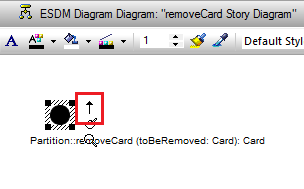
\includegraphics[width=0.5\textwidth]{ea_activateQuickLink}
  \caption{Quick link in SDM diagram to create new activity node {\bf update}}  
  \label{fig:sdm_quicklink}
\end{center}
\end{figure}

\item[$\blacktriangleright$] EA notices that there is nothing to quick-link to, and pops up a small context-sensitive dialogue to create an element that can be
connected to the indicated source element.

\item[$\blacktriangleright$] As indicated in Fig.~\ref{fig:sdm_new_activity_node}, choose \texttt{Append StoryNode} to create an \emph{activity
node}.\define{Activity~Node}We shall refer to the whole activity diagram simply as an \emph{activity}\define{Activity} that always starts with a start node,
terminates with a \emph{stop node}, and consists of activity nodes connected via \emph{activity edges}.\define{Activity~Edge}If you quick created correctly,
you should now have a start node, an activity node called \texttt{ActivityNode 1}, and an edge connecting the start node to the activity node.

\begin{figure}[htp]
\begin{center}
  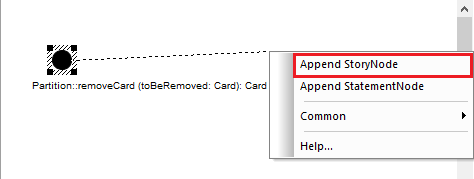
\includegraphics[width=0.8\textwidth]{ea_quickLinkStoryNode}
  \caption{Create new activity node {\bf update}}  
  \label{fig:sdm_new_activity_node}
\end{center}
\end{figure}

\item[$\blacktriangleright$] Complete the activity by quick creating a stop node as depicted in Fig.~\ref{fig:sdm_stop_node}.

\begin{figure}[htp]
\begin{center}
  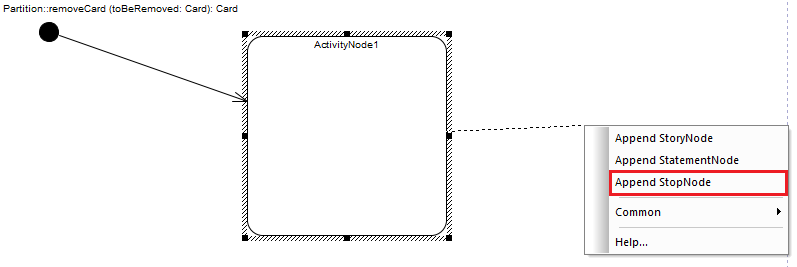
\includegraphics[width=\textwidth]{ea_appendStop}
  \caption{Complete activity with a stop node {\bf update}}  
  \label{fig:sdm_stop_node}
\end{center}
\end{figure}

\item[$\blacktriangleright$] If everything is correct, you should now have a complete activity that models the procedural \emph{control flow} of our method. 
The semantics of our activities is pretty straightforward -- the control flow starts in the start node and flows along edges and connected activity nodes until
it terminates in a stop node. The complete activity is depicted in Fig.~\ref{fig:sdm_complete_control_flow_simple} now with the activity node connected via
an activity edge to the newly created stop node.

\label{story-pattern}
Integrated as an atomic step in this overall control flow, a single graph transformation step can be embedded in some activity nodes as a
\emph{story pattern}.\define{Story~Patte\-rn}These story patterns are declarative transformation rules as introduced in Part II while discussing static
semantics. As not all activity nodes can contain story patterns (e.g. start and stop nodes), those that can are called \emph{story nodes}\define{Story~Nodes}.

\begin{figure}[htp]
\begin{center}
  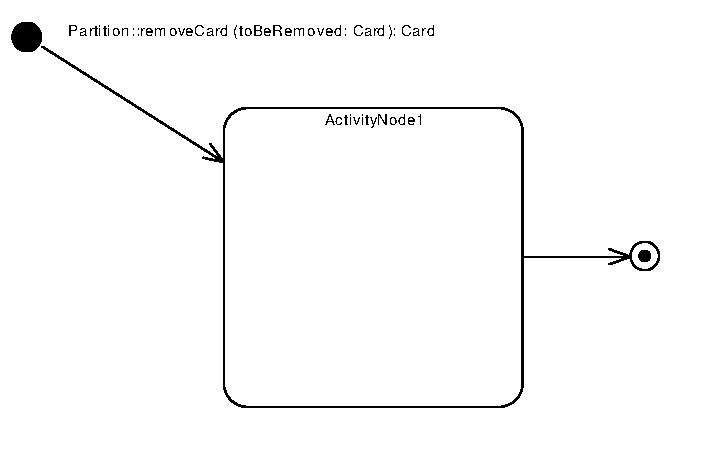
\includegraphics[width=0.7\textwidth]{ea_controlFlowRemoveCard.pdf}
  \caption{Control flow modelled as a simple activity diagram {\bf update}}  
  \label{fig:sdm_complete_control_flow_simple}
\end{center}
\end{figure}

\item[$\blacktriangleright$] To create a story pattern, double click the \texttt{ActivityNode 1} story node (Fig.~\ref{fig:sdm_complete_control_flow_simple}) to
prompt the dialogue depicted in Fig.~\ref{fig:story_pattern}.

\item[$\blacktriangleright$] Enter \texttt{remove\-Card\-From\-Partition} as the name of the story node, check \texttt{Create this Object} and click
\texttt{OK}.

\begin{figure}[htpb]
\begin{center} 
  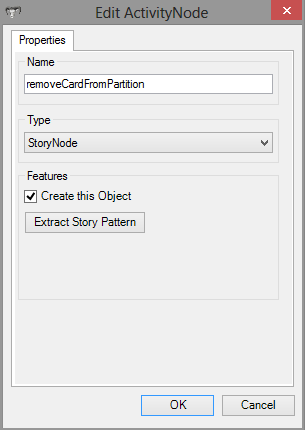
\includegraphics[width=0.45\textwidth]{ea_createStoryNode}
  \caption{Start modelling story pattern in activity node}  
  \label{fig:story_pattern}
\end{center}
\end{figure}

The activity node should now have a single \emph{object variable},\define{Object~Variable}\texttt{this} (Fig.~\ref{fig:tool_box}). Object variables are, as
the word ``variable'' indicates, place holders for actual objects in a model.  During \emph{pattern matching}, actual objects in the 
current model are assigned to the object variables in the pattern according to  the indicated type of the object variable and other conditions\footnote{We shall
learn what conditions can be specified in a few pages.}.  In our case, the current story pattern consists of only one object variable, which is assigned (per
convention) to \texttt{this} in Java (the object whose method is invoked).

\begin{figure}[htp]
\begin{center}
  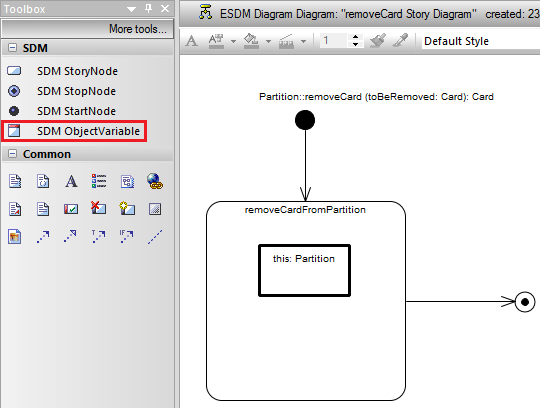
\includegraphics[width=0.8\textwidth]{ea_sdmNewObjVar}
  \caption{Add a new object variable from the tool-box {\bf update}}  
  \label{fig:tool_box}
\end{center}
\end{figure}

\item[$\blacktriangleright$] To create an object variable that can be assigned to other objects, choose \texttt{SDM ObjectVariable} from the toolbox as
indicated in Fig.~\ref{fig:tool_box} and click \emph{in} the activity node \texttt{removeCardFromPartition} (Fig.~\ref{fig:object_variable_properties}).

\begin{figure}[htp]
\begin{center}
  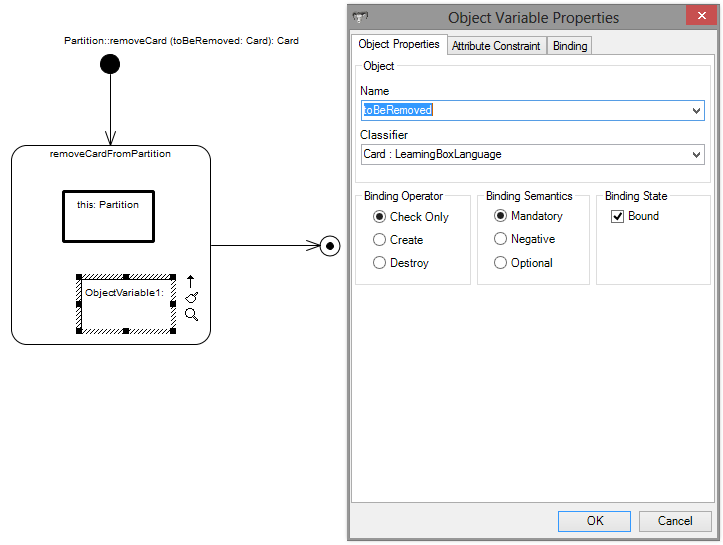
\includegraphics[width=0.8\textwidth]{ea_propertiesObjVar}
  \caption{Specify properties of the added object variable {\bf update}}  
  \label{fig:object_variable_properties}
\end{center}
\end{figure}

\item[$\blacktriangleright$] In the dialogue that pops up, choose \texttt{toBeRemoved} as the name of the object variable and \texttt{Card} as its type using
the corresponding drop-down menus. Because \texttt{toBeRemoved} is a parameter of the method, it is offered as a possible name in the drop-down menu and can be
directly chosen to prevent annoying mistakes due to typing the name of the parameter incorrectly.

In this dialogue, note that the option \texttt{Bound} that must be set. For the pattern matcher, bound object variables do not need
to be assigned as they already have a fixed value from the context of the method.   We have already seen two cases  for bound object variables: the assignment
to \texttt{this} (the current partition who owns the method), and assignments to parameters of the method that  are specified when invoking
the method.   Please note that the assignment or \emph{binding [state]}\define{Binding~State} is in both cases implicit and via the \emph{name} of the bound
object variable.

\begin{figure}[htp]
\begin{center}
  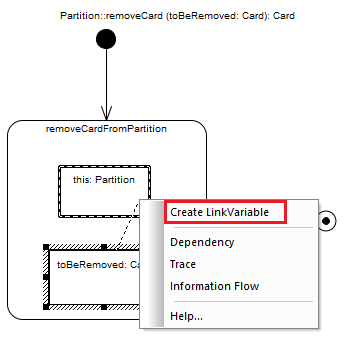
\includegraphics[width=0.55\textwidth]{ea_createLinkVar}
  \caption{Create a link variable {\bf update}}   
  \label{fig:link_variable}
\end{center}
\end{figure}

Knowing that models consist not only of objects, but also of \emph{links}, one can create \emph{link variables}\define{Link~Variab\-le} to match links in story
patterns that act as place holders for links in a model.

\item[$\blacktriangleright$] To create a link variable between the current partition, whose \texttt{removeCard} method is invoked, and the
card to be removed, which is passed in as a parameter of the method, choose the object variable \texttt{this} and quick link it to the object variable
\texttt{toBeRemoved}. In the quick link dialogue, choose \texttt{Create LinkVariable} (Fig.~\ref{fig:link_variable}).

\item[$\blacktriangleright$] In the property dialogue that pops up, choose the offered link type (according to the metamodel, there is only one possible link
type between a partition and a card), and set the \emph{Binding Operator}\define{Binding~Operator} to \texttt{Destroy}
(Fig.~\ref{fig:link_variable_properties}). Every object or link variable's binding operator can be set to one of \texttt{Check Only, Create, Destroy}.

\begin{figure}[htp]
\begin{center} 
 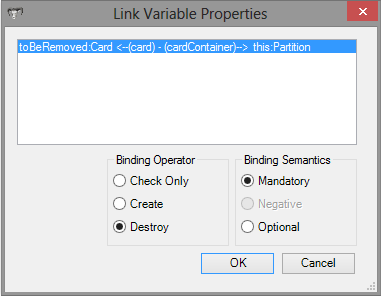
\includegraphics[width=0.6\textwidth]{ea_propertiesLinkVar}
  \caption{Specify properties for created link variable}  
  \label{fig:link_variable_properties}
\end{center}
\end{figure}

For a rule $r: (L, R)$, as discussed at the beginning of this Part III, this marks the variable as belonging to the set of elements to be retained ($L\cap R$), the
set of elements to be newly created ($R\setminus L$), or the set of elements to be deleted ($L\setminus R$).

\item[$\blacktriangleright$] Remember how we said that this method should return the passed in card? As luck would have it, a return value for any SDM can be
specified in the stop node. As depicted in Fig.~\ref{fig:stop_node_return_value}, double-click the stop node to prompt the \texttt{Edit StopNode} dialogue. 

\item[$\blacktriangleright$] In the \texttt{Expression} field, choose \texttt{ParameterExpression}, and \texttt{toBeRemoved} as the parameter.

\begin{figure}[htp]
\begin{center}
  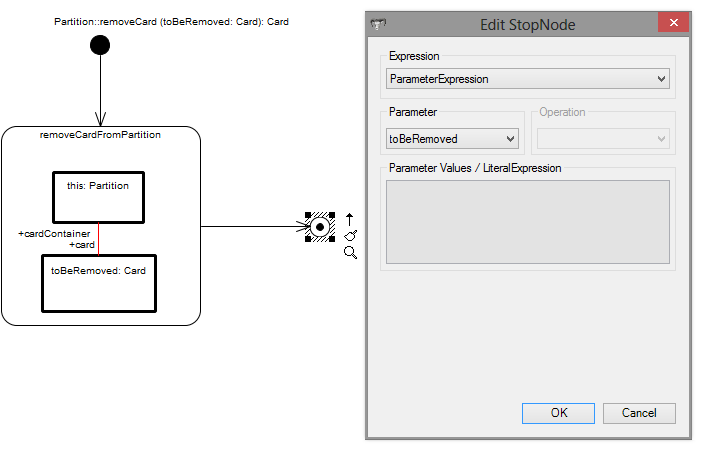
\includegraphics[width=0.95\textwidth]{ea_editStopNode}
  \caption{Adding a return value to the stop node {\bf update}}  
  \label{fig:stop_node_return_value}
\end{center}
\end{figure}

In many different dialogues, eMoflon employs a simple context-sensitive expression language for specifying required values. We have intentionally
avoided creating a full-blown sub-language, and limit expressions to a few simple types\footnote{We also do not support nesting expressions.}. The philosophy here
is to keep things simple and concentrate on what SDMs are good for -- expressing structural change. Our approach is to provide a clear and type-safe interface
to a general purpose language (Java) and support a simple \emph{fallback} as soon as things get low-level and difficult to express as a pattern.

The alternative approach to eMoflon would be to support arbitrary expressions, for example, in a script language like JavaScript or in an appropriate
DSL\footnote{A DSL is a Domain Specific Language: a language designed for a specific task which is usually simpler than a general purpose language like Java and
more suitable for the exact task.} designed for this purpose. In the following SDM implementations, we'll learn the other expression types eMoflon supports,
and how to use them. For the moment however, we'll use a \emph{ParameterExpression}\define{ParameterExpr\-ession}which refers to the parameters of the current
method, exactly what we needed and have used for our \texttt{removeCard} SDM.

\item[$\blacktriangleright$] If you've done everything right, your complete SDM should now look like Fig.~\ref{fig:sdm_complete_control_flow}, with the return
value indicated below the stop node.

\item[$\blacktriangleright$] Let's take a step back and review briefly what we have specified:  if \texttt{p.remove\-Card(c)} is invoked for a partition
\texttt{p}, with a card \texttt{c} as its argument, the specified pattern will \emph{match} if that card is contained in the partition. After determining this
match for all variables, the link between the partition and the card is deleted, effectively ``removing'' the card from the partition. If the card is \emph{not}
contained in the partition, the pattern won't match and nothing will happen. In both cases, the card that was passed in is returned.

\vspace{1cm}
\begin{figure}[htbp]
\begin{center}
  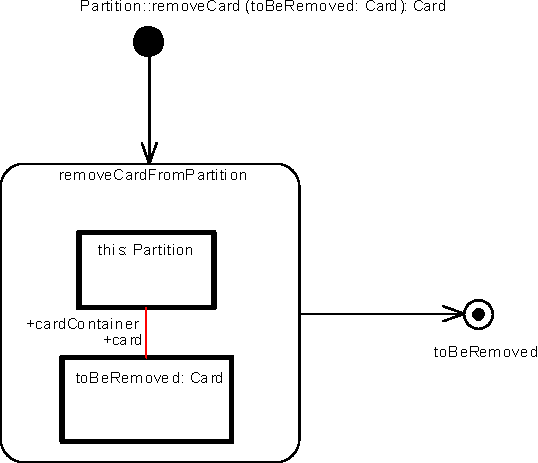
\includegraphics[width=0.7\textwidth]{ea_completeSDMRemoveCard.pdf}
  \caption{Complete SDM for \texttt{Partition::removeCard}}  
  \label{fig:sdm_complete_control_flow}
\end{center}
\end{figure}

\item[$\blacktriangleright$] Congratulations! You have completely specified your first SDM using eMolfon! Don't forget to export and generate your code in the
Eclipse workspace \footnote{Go to to ``\texttt{Extensions}" and select \texttt{Add-In Windows} to activate eMoflon's console - the \texttt{Export} options
should be available there.If you're unsure how to validate, export, or use this window, review Part II, section \#}. In the following sections, we shall explore
further features of SDM that allow for really expressive and powerful patterns.

\item[$\blacktriangleright$] Inspect the generated implementation for your method\footnote{The generated method is in
\texttt{/Learning\-Box\-Language/\-gen/\-Learning\-Box\-Language/\-impl/\-Partition\-Impl.java/\-remove\-Card}}, and see if you can get a feel for what the
generated code does. Notice all the null checks that are automatically created - only a very conscientious (and probably slightly paranoid) programmer would
program so defensively!

\item[$\blacktriangleright$] If you're unable to export or generate code successfully, compare your SDM carefully with Fig.~\ref{fig:sdm_complete_control_flow}
and make sure you haven't forgotten anything.

\item[$\blacktriangleright$] If you'd like to see how \texttt{removeCard} is implemented in the textual syntax, skip the link below, and proceed to the
next page. Continue to learn how to implement \texttt{checkCard}.

\fancyfoot[R]{ $\triangleright$ \hyperlink{sec:checkCard}{Next} }

\end{itemize}

